% Options for packages loaded elsewhere
\PassOptionsToPackage{unicode}{hyperref}
\PassOptionsToPackage{hyphens}{url}
%
\documentclass[
]{article}
\usepackage{amsmath,amssymb}
\usepackage{iftex}
\ifPDFTeX
  \usepackage[T1]{fontenc}
  \usepackage[utf8]{inputenc}
  \usepackage{textcomp} % provide euro and other symbols
\else % if luatex or xetex
  \usepackage{unicode-math} % this also loads fontspec
  \defaultfontfeatures{Scale=MatchLowercase}
  \defaultfontfeatures[\rmfamily]{Ligatures=TeX,Scale=1}
\fi
\usepackage{lmodern}
\ifPDFTeX\else
  % xetex/luatex font selection
\fi
% Use upquote if available, for straight quotes in verbatim environments
\IfFileExists{upquote.sty}{\usepackage{upquote}}{}
\IfFileExists{microtype.sty}{% use microtype if available
  \usepackage[]{microtype}
  \UseMicrotypeSet[protrusion]{basicmath} % disable protrusion for tt fonts
}{}
\makeatletter
\@ifundefined{KOMAClassName}{% if non-KOMA class
  \IfFileExists{parskip.sty}{%
    \usepackage{parskip}
  }{% else
    \setlength{\parindent}{0pt}
    \setlength{\parskip}{6pt plus 2pt minus 1pt}}
}{% if KOMA class
  \KOMAoptions{parskip=half}}
\makeatother
\usepackage{xcolor}
\usepackage[margin=1in]{geometry}
\usepackage{longtable,booktabs,array}
\usepackage{calc} % for calculating minipage widths
% Correct order of tables after \paragraph or \subparagraph
\usepackage{etoolbox}
\makeatletter
\patchcmd\longtable{\par}{\if@noskipsec\mbox{}\fi\par}{}{}
\makeatother
% Allow footnotes in longtable head/foot
\IfFileExists{footnotehyper.sty}{\usepackage{footnotehyper}}{\usepackage{footnote}}
\makesavenoteenv{longtable}
\usepackage{graphicx}
\makeatletter
\def\maxwidth{\ifdim\Gin@nat@width>\linewidth\linewidth\else\Gin@nat@width\fi}
\def\maxheight{\ifdim\Gin@nat@height>\textheight\textheight\else\Gin@nat@height\fi}
\makeatother
% Scale images if necessary, so that they will not overflow the page
% margins by default, and it is still possible to overwrite the defaults
% using explicit options in \includegraphics[width, height, ...]{}
\setkeys{Gin}{width=\maxwidth,height=\maxheight,keepaspectratio}
% Set default figure placement to htbp
\makeatletter
\def\fps@figure{htbp}
\makeatother
\setlength{\emergencystretch}{3em} % prevent overfull lines
\providecommand{\tightlist}{%
  \setlength{\itemsep}{0pt}\setlength{\parskip}{0pt}}
\setcounter{secnumdepth}{5}
\usepackage{booktabs}
\usepackage{longtable}
\usepackage{array}
\usepackage{multirow}
\usepackage{wrapfig}
\usepackage{float}
\usepackage{colortbl}
\usepackage{pdflscape}
\usepackage{tabu}
\usepackage{threeparttable}
\usepackage{threeparttablex}
\usepackage[normalem]{ulem}
\usepackage{makecell}
\usepackage{xcolor}
\ifLuaTeX
  \usepackage{selnolig}  % disable illegal ligatures
\fi
\IfFileExists{bookmark.sty}{\usepackage{bookmark}}{\usepackage{hyperref}}
\IfFileExists{xurl.sty}{\usepackage{xurl}}{} % add URL line breaks if available
\urlstyle{same}
\hypersetup{
  pdftitle={Aggregating Anteaters Project},
  hidelinks,
  pdfcreator={LaTeX via pandoc}}

\title{Aggregating Anteaters Project}
\author{}
\date{\vspace{-2.5em}2023-11-16}

\begin{document}
\maketitle

{
\setcounter{tocdepth}{2}
\tableofcontents
}
\hypertarget{data-preparation}{%
\section{Data Preparation}\label{data-preparation}}

Before describing the data, we conducted some initial checks to ensure that all observations were entered within their possible ranges (for continuous variables) or levels (for categorical variables). We used some initial visualisations of the marginal distributions and relationships amongst the variables to find these impossible values (see Figure \ref{fig:ini-pairs-panels} for these for the pre-processed data in the Appendix). We excluded impossible values along with any observation containing missing data (N\textsubscript{excluded} = 5). Table \ref{tab:excl-tab} in the Appendix provides an overview of these excluded data points and the reason for exclusion. Additionally, the spelling of ``Apple'' was corrected in the operating system entry of 7 observations from ``Appple''.

\hypertarget{data-description}{%
\section{Data Description}\label{data-description}}

\hypertarget{association-between-operating-system-and-frequency-of-emoji-use-julie-and-ella}{%
\subsection{Association Between Operating System and Frequency of Emoji Use (Julie and Ella)}\label{association-between-operating-system-and-frequency-of-emoji-use-julie-and-ella}}

We explored whether there's a difference in the frequency of emoji use between Apple and Android users. We did this in two ways - we created violin plots, and conducted a Welch two sample t-test.

From Figure \ref{fig:q1b-violin-plot}, we can see that the lower quartile and median of the two operating systems are very similar. However, the upper quartile is higher and overall range is larger for Apple than Android. It seems that Apple users seem more likely to use a higher number of emojis per day. Android users, however, are more densely concentrated around the median. In the data set, we can see there is only one outlier - at 24 emojis per day for one Apple user.

\begin{figure}
\centering
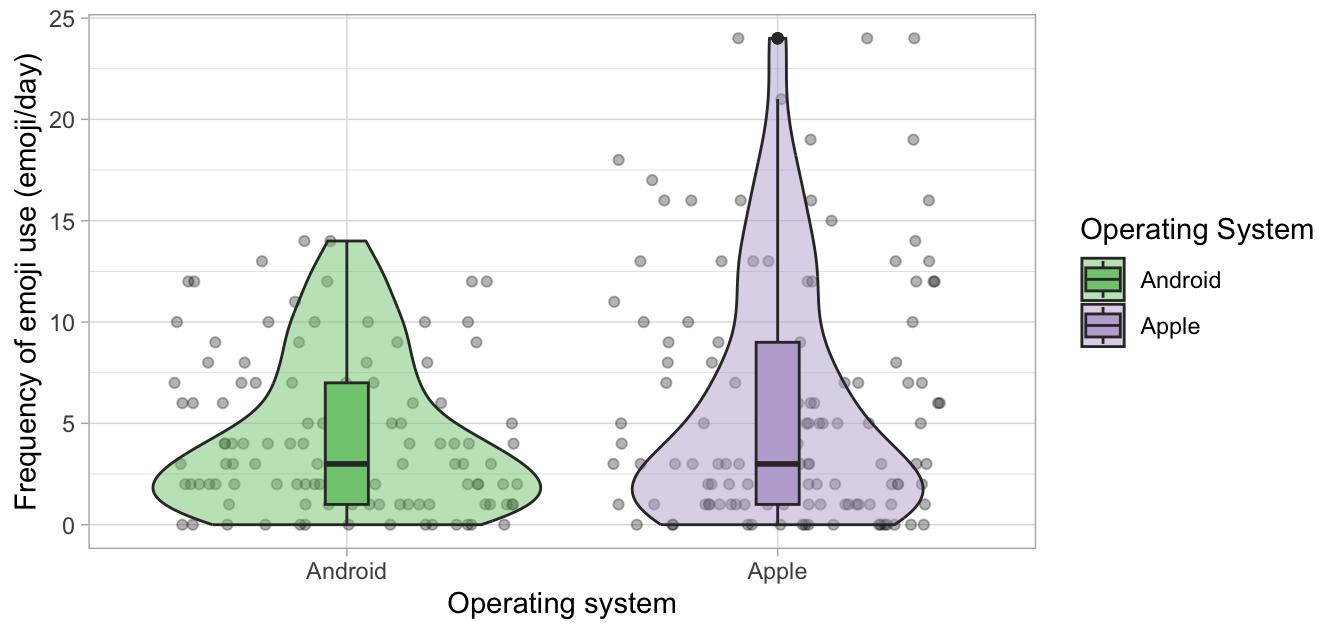
\includegraphics{Anteaters_Group_Project_files/figure-latex/q1b-violin-plot-1.pdf}
\caption{\label{fig:q1b-violin-plot}Frequency of Emoji Use on Apple and Android Operating System}
\end{figure}

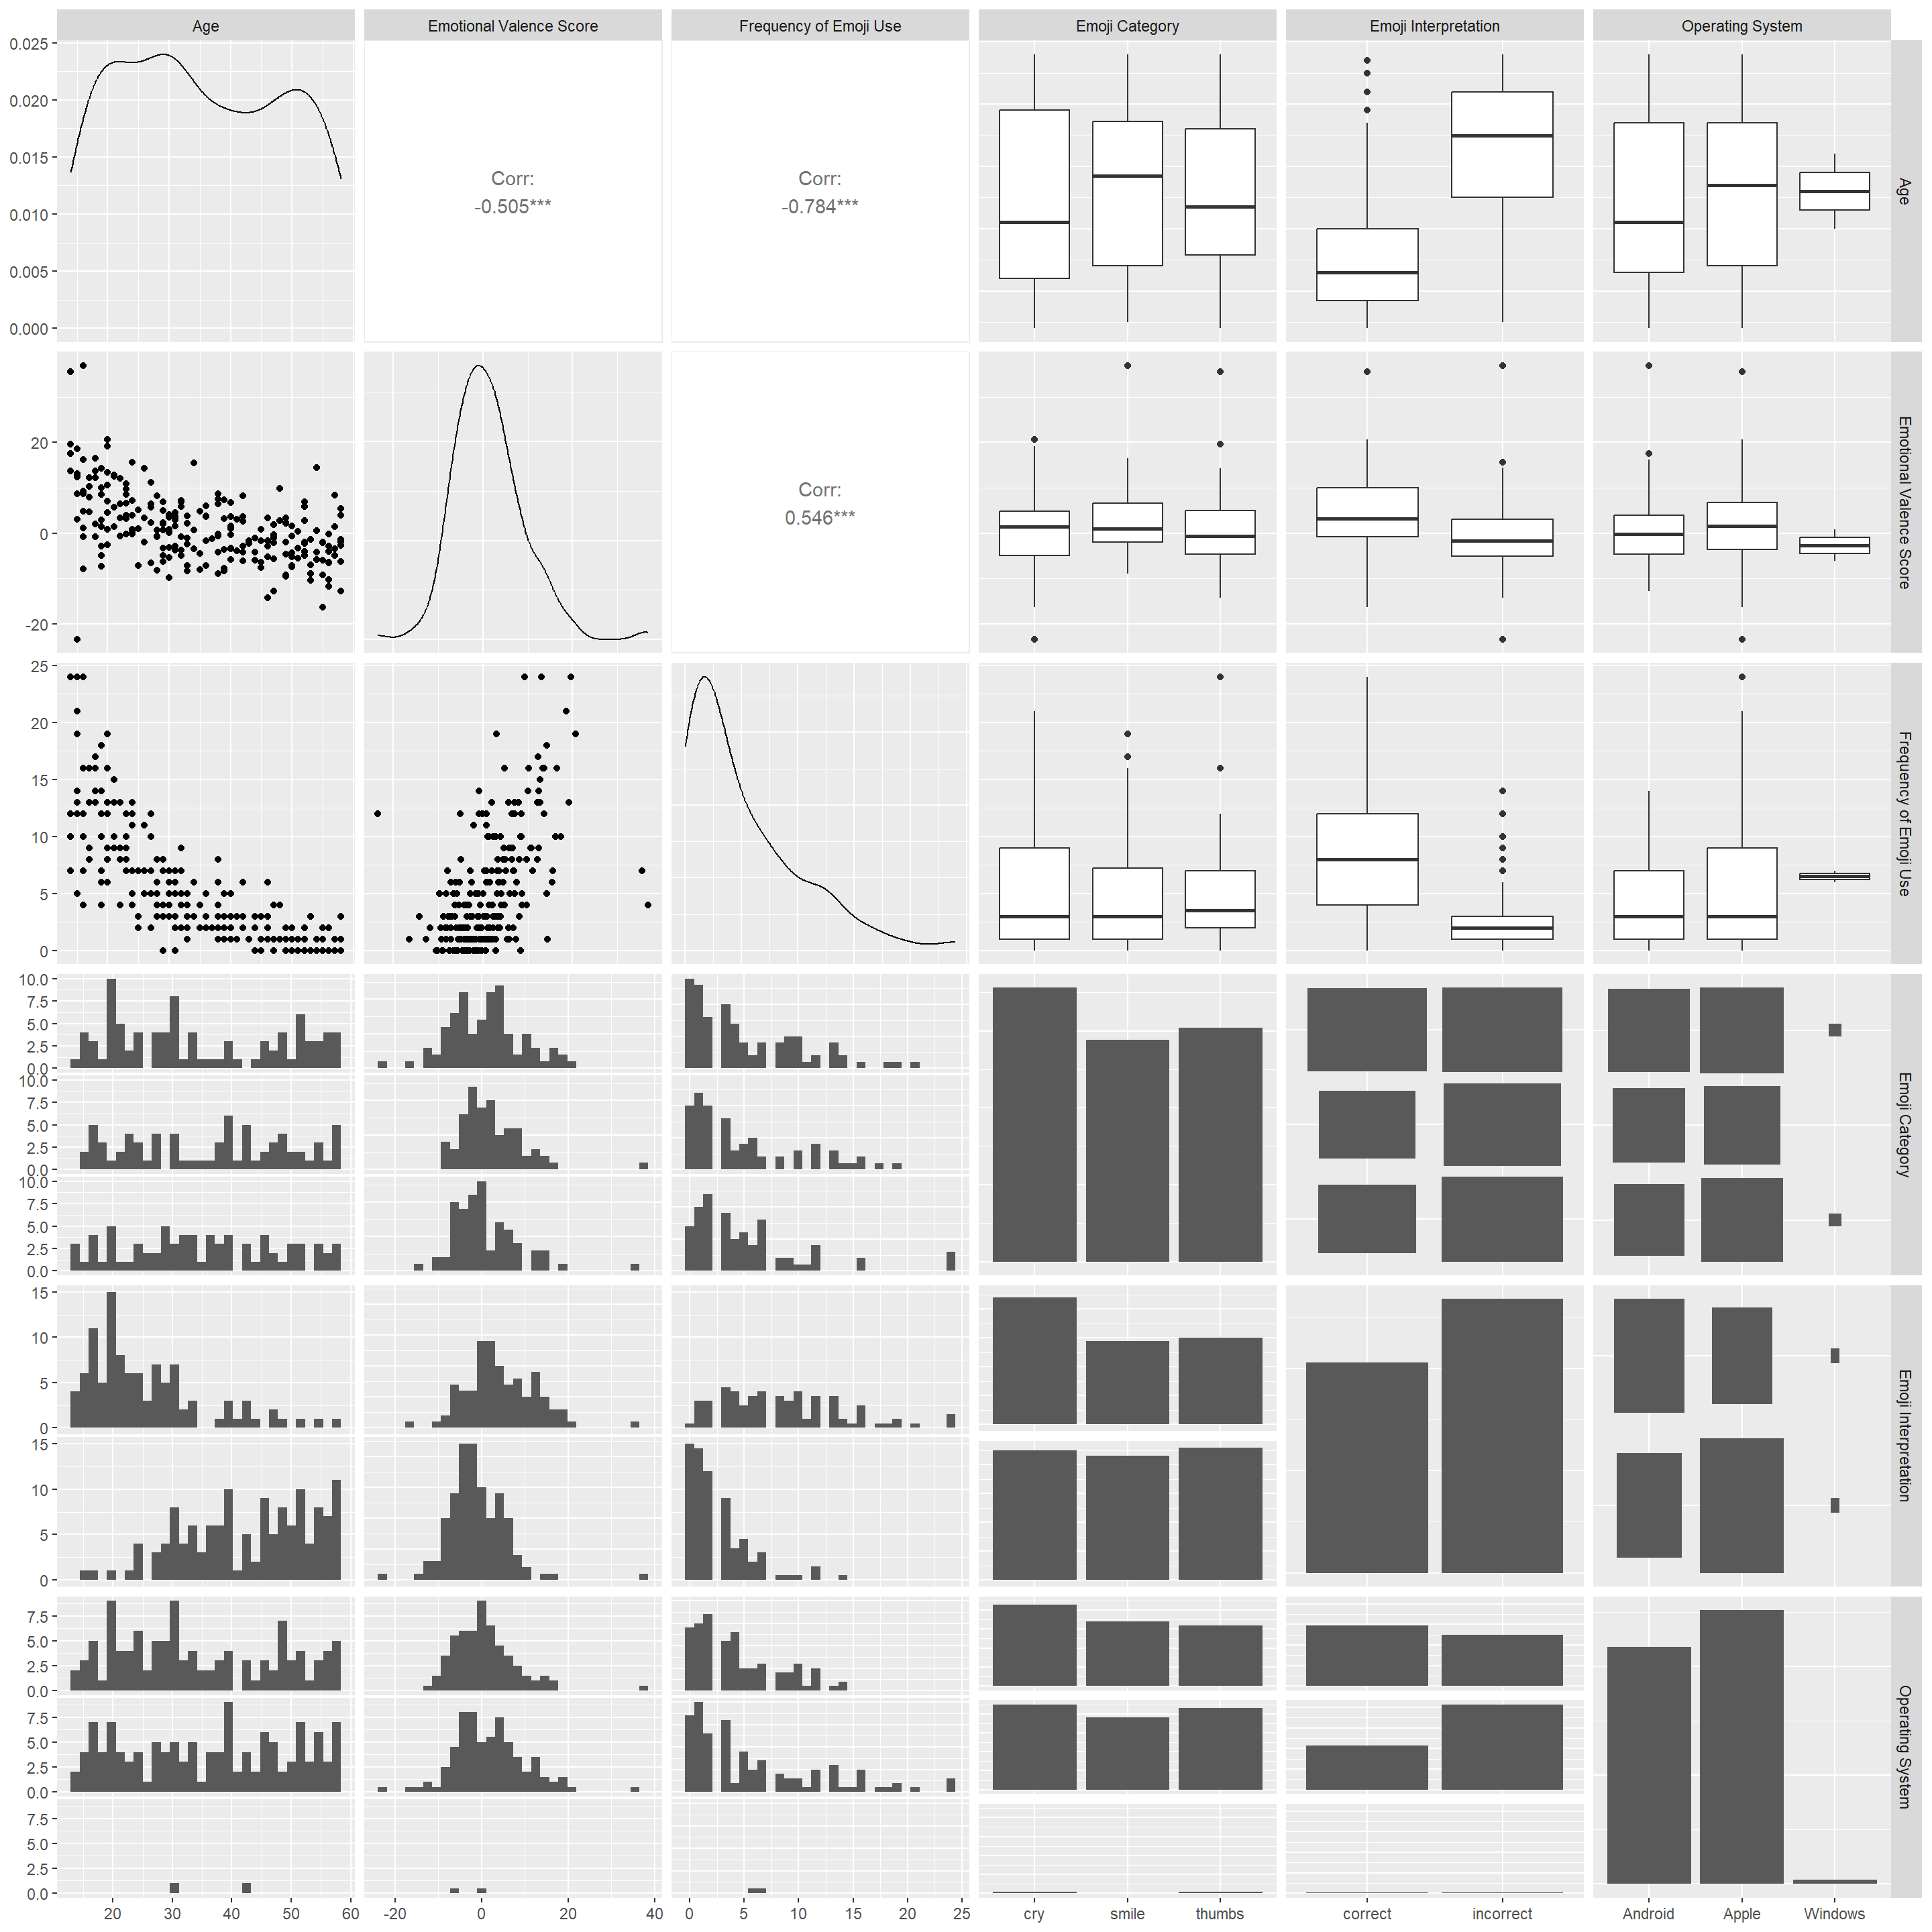
\includegraphics{Anteaters_Group_Project_files/figure-latex/unnamed-chunk-1-1.pdf}

Following this, we conducted a Welch two sample t-test to assess whether the mean frequency of emoji use was different between Android (\emph{n} = 109 ; \emph{m} = 4.3; \emph{sd} = 3.77 and Apple users (\emph{n} = 126; \emph{m} = 5.87; \emph{sd} = 6.01). There was a significant difference in emoji use among Android and Apple users, \emph{t}(213.42) = -2.39, \emph{p} = 0.018, two-tailed).Therefore, we reject the null hypothesis that there is no difference in emoji use between Apple and Android users. From these two mechanisms, we have concluded that there is a difference between the two operating systems.

\hypertarget{correlation-between-age-and-frequency-of-emoji-use-renia}{%
\subsection{Correlation Between Age and Frequency of Emoji Use (Renia)}\label{correlation-between-age-and-frequency-of-emoji-use-renia}}

\textbf{To do}

\begin{itemize}
\tightlist
\item
  Introduction to the test
\item
  plot commentary
\item
  solution for non-normality
\end{itemize}

\begin{figure}
\centering
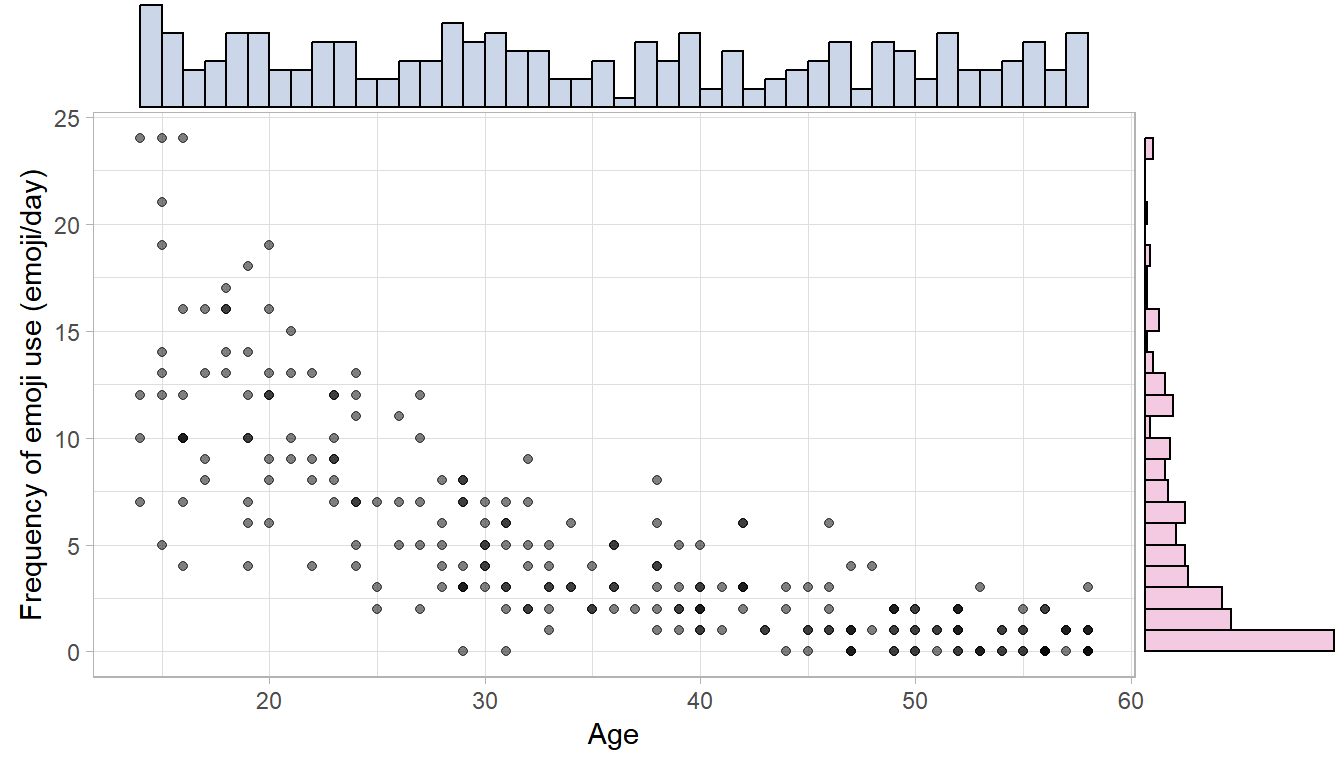
\includegraphics{Anteaters_Group_Project_files/figure-latex/cor-plot-1.pdf}
\caption{\label{fig:cor-plot}Relationship Between Age and Frequency of Emoji Use}
\end{figure}

Correlation test Interpretation

A correlation test was conducted to assess whether there is a relationship between the age of an individual, and the frequency by which they use emoji. A total of 237 individuals were included in the analysis, with a mean age of 35.39 (\emph{sd} = 13.4) and a mean frequency of use of emoji of 5.16 (\emph{sd} = 5.13).There was a strong negative correlation between age of an individual and the frequency of emoji use (\emph{r} = -0.78, \emph{t}(235) = -19.39), \emph{p} \textless{} 0.001. We therefore reject the null hypothesis that there is no correlation between age and frequency of emoji use. Figure 1 provides a visualization of the relationship.

\hypertarget{balance-of-users-of-operating-systems-for-emoji-categories-meg-and-julie}{%
\subsection{Balance of Users of Operating Systems for Emoji Categories (Meg and Julie)}\label{balance-of-users-of-operating-systems-for-emoji-categories-meg-and-julie}}

\textbf{To do}

\begin{itemize}
\tightlist
\item
  plot commentary
\end{itemize}

\begin{figure}
\centering
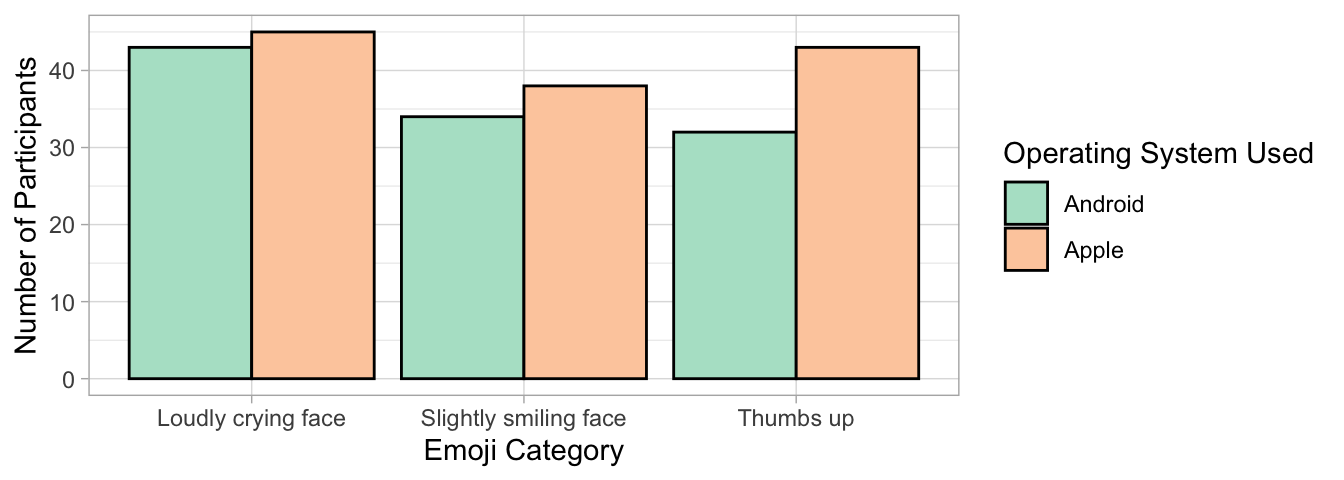
\includegraphics{Anteaters_Group_Project_files/figure-latex/q1c-bar-plot-1.pdf}
\caption{\label{fig:q1c-bar-plot}Distribution of Participants on Apple and Android Operating System for Each Emoji Category}
\end{figure}

Finally, we investigated whether there is a balance between Apple and Android users for each category of emoji. We conducted a \(\chi^2\) goodness of fit test for each emoji category, which tests if the observed proportion of participants using Apple and Android deviates from hypothesised equal proportions of users (50\% of the data each) indicating balance.

For each emoji category, we found no significant difference between the observed proportions of Apple and Android users, and a hypothesised set of equal proportions. For loudly crying face emoji {[}😭{]}, \(\chi^2\) (1) = 0.05, \emph{p} = 0.831 (\emph{n} = 88, \emph{proportion\textsubscript{Apple}} = 51.14 \%, \emph{proportion\textsubscript{Android}} = 48.86 \%). For the slightly smiling face emoji {[}🙂{]}, \(\chi^2\) (1) = 0.22, \emph{p} = 0.637 (\emph{n} = 72, \emph{proportion\textsubscript{Apple}} = 52.78 \%, \emph{proportion\textsubscript{Android}} = 47.22 \%). Finally, for the thumbs up Emoji {[}👍{]}, \(\chi^2\) (1) = 1.61, \emph{p} = 0.204 (\emph{n} = 75, \emph{proportion\textsubscript{Apple}} = 57.33 \%, \emph{proportion\textsubscript{Android}} = 42.67 \%). Thus, we found no evidence of imbalance of users of Apple and Android operated phones in each emoji category.

\hypertarget{the-emotional-effect-of-emojis-renia-meg}{%
\section{The Emotional Effect of Emojis (Renia \& Meg)}\label{the-emotional-effect-of-emojis-renia-meg}}

\textbf{To do}
* generate relevant plots
* plot commentary
* check assumptions
* check for multicolinearity
* check for influential values

One of the main aims we address in this research is the investigation of factors influencing emotional valence. We fitted a multiple regression model to predict whether the type of emoji and the frequency of use of the emoji, as well as the age of the participants, has an effect on their emotional valence. We mean-centered age for interpretation of coefficients and intercepts.

thumbs up regression coef: -0.54
interaction term: 0.04

\hypertarget{accuracy-of-emoji-interpretation-julie}{%
\section{Accuracy of Emoji Interpretation (Julie)}\label{accuracy-of-emoji-interpretation-julie}}

\textbf{To do}

\begin{itemize}
\tightlist
\item
  include maximum likelihood estimation
\item
  comment on previous results
\item
  Comment on plots
\item
  check influential values
\item
  finish write-up
\end{itemize}

Finally, we address the research aim of what factors make participants more or less likely to correctly interpret Emoji (according to the researchers' coding scheme). The predictors of interest were the same as the previous regression model;frequency of emoji use first as its effect on interpreting Emoji is already known, and additionally age and Emoji category along with the interaction between these to investigate if the effect of age on interpretation accuracy is dependent on the Emoji being interpreted. Figure \ref{fig:q3-desc-plots} provides an overview of the marginal distributions of these variables (Figures \ref{fig:q3-desc-plots}C-E) and the relationships with Emoji interpretation accuracy for age by Emoji category (Figure \ref{fig:q3-desc-plots}A) and for frequency of Emoji use (Figure \ref{fig:q3-desc-plots}B). As noted previously, neither age (approximately uniform; Figure \ref{fig:q3-desc-plots}C) nor frequency of Emoji use (approximately Poison distributed; Figure \ref{fig:q3-desc-plots}D) were normally distributed, and there were slightly more participants who interpreted the loudly crying face Emoji {[}😭{]} than the other Emoji categories(Figure \ref{fig:q3-desc-plots}D). Generally, a slightly higher proportion of participants interpreted their Emoji incorrectly as compared to correct interpretations (Figures \ref{fig:q3-desc-plots}E). Examining the median age and frequency in Figures \ref{fig:q3-desc-plots}A-B, it seems that incorrect responses are more common for participants with higher age and lower frequency use. Although correct responses were more evenly distributed across frequency of Emoji use relative to incorrect responses, which tended to be below five Emoji per day. Figure \ref{fig:q3-desc-plots}A provided some indication that the Emoji being interpreted may moderate the relationship between lower age for correct interpretations - specifically, that the thumbs up Emoji {[}👍{]} seem to have slightly lower median age for correct interpretations.

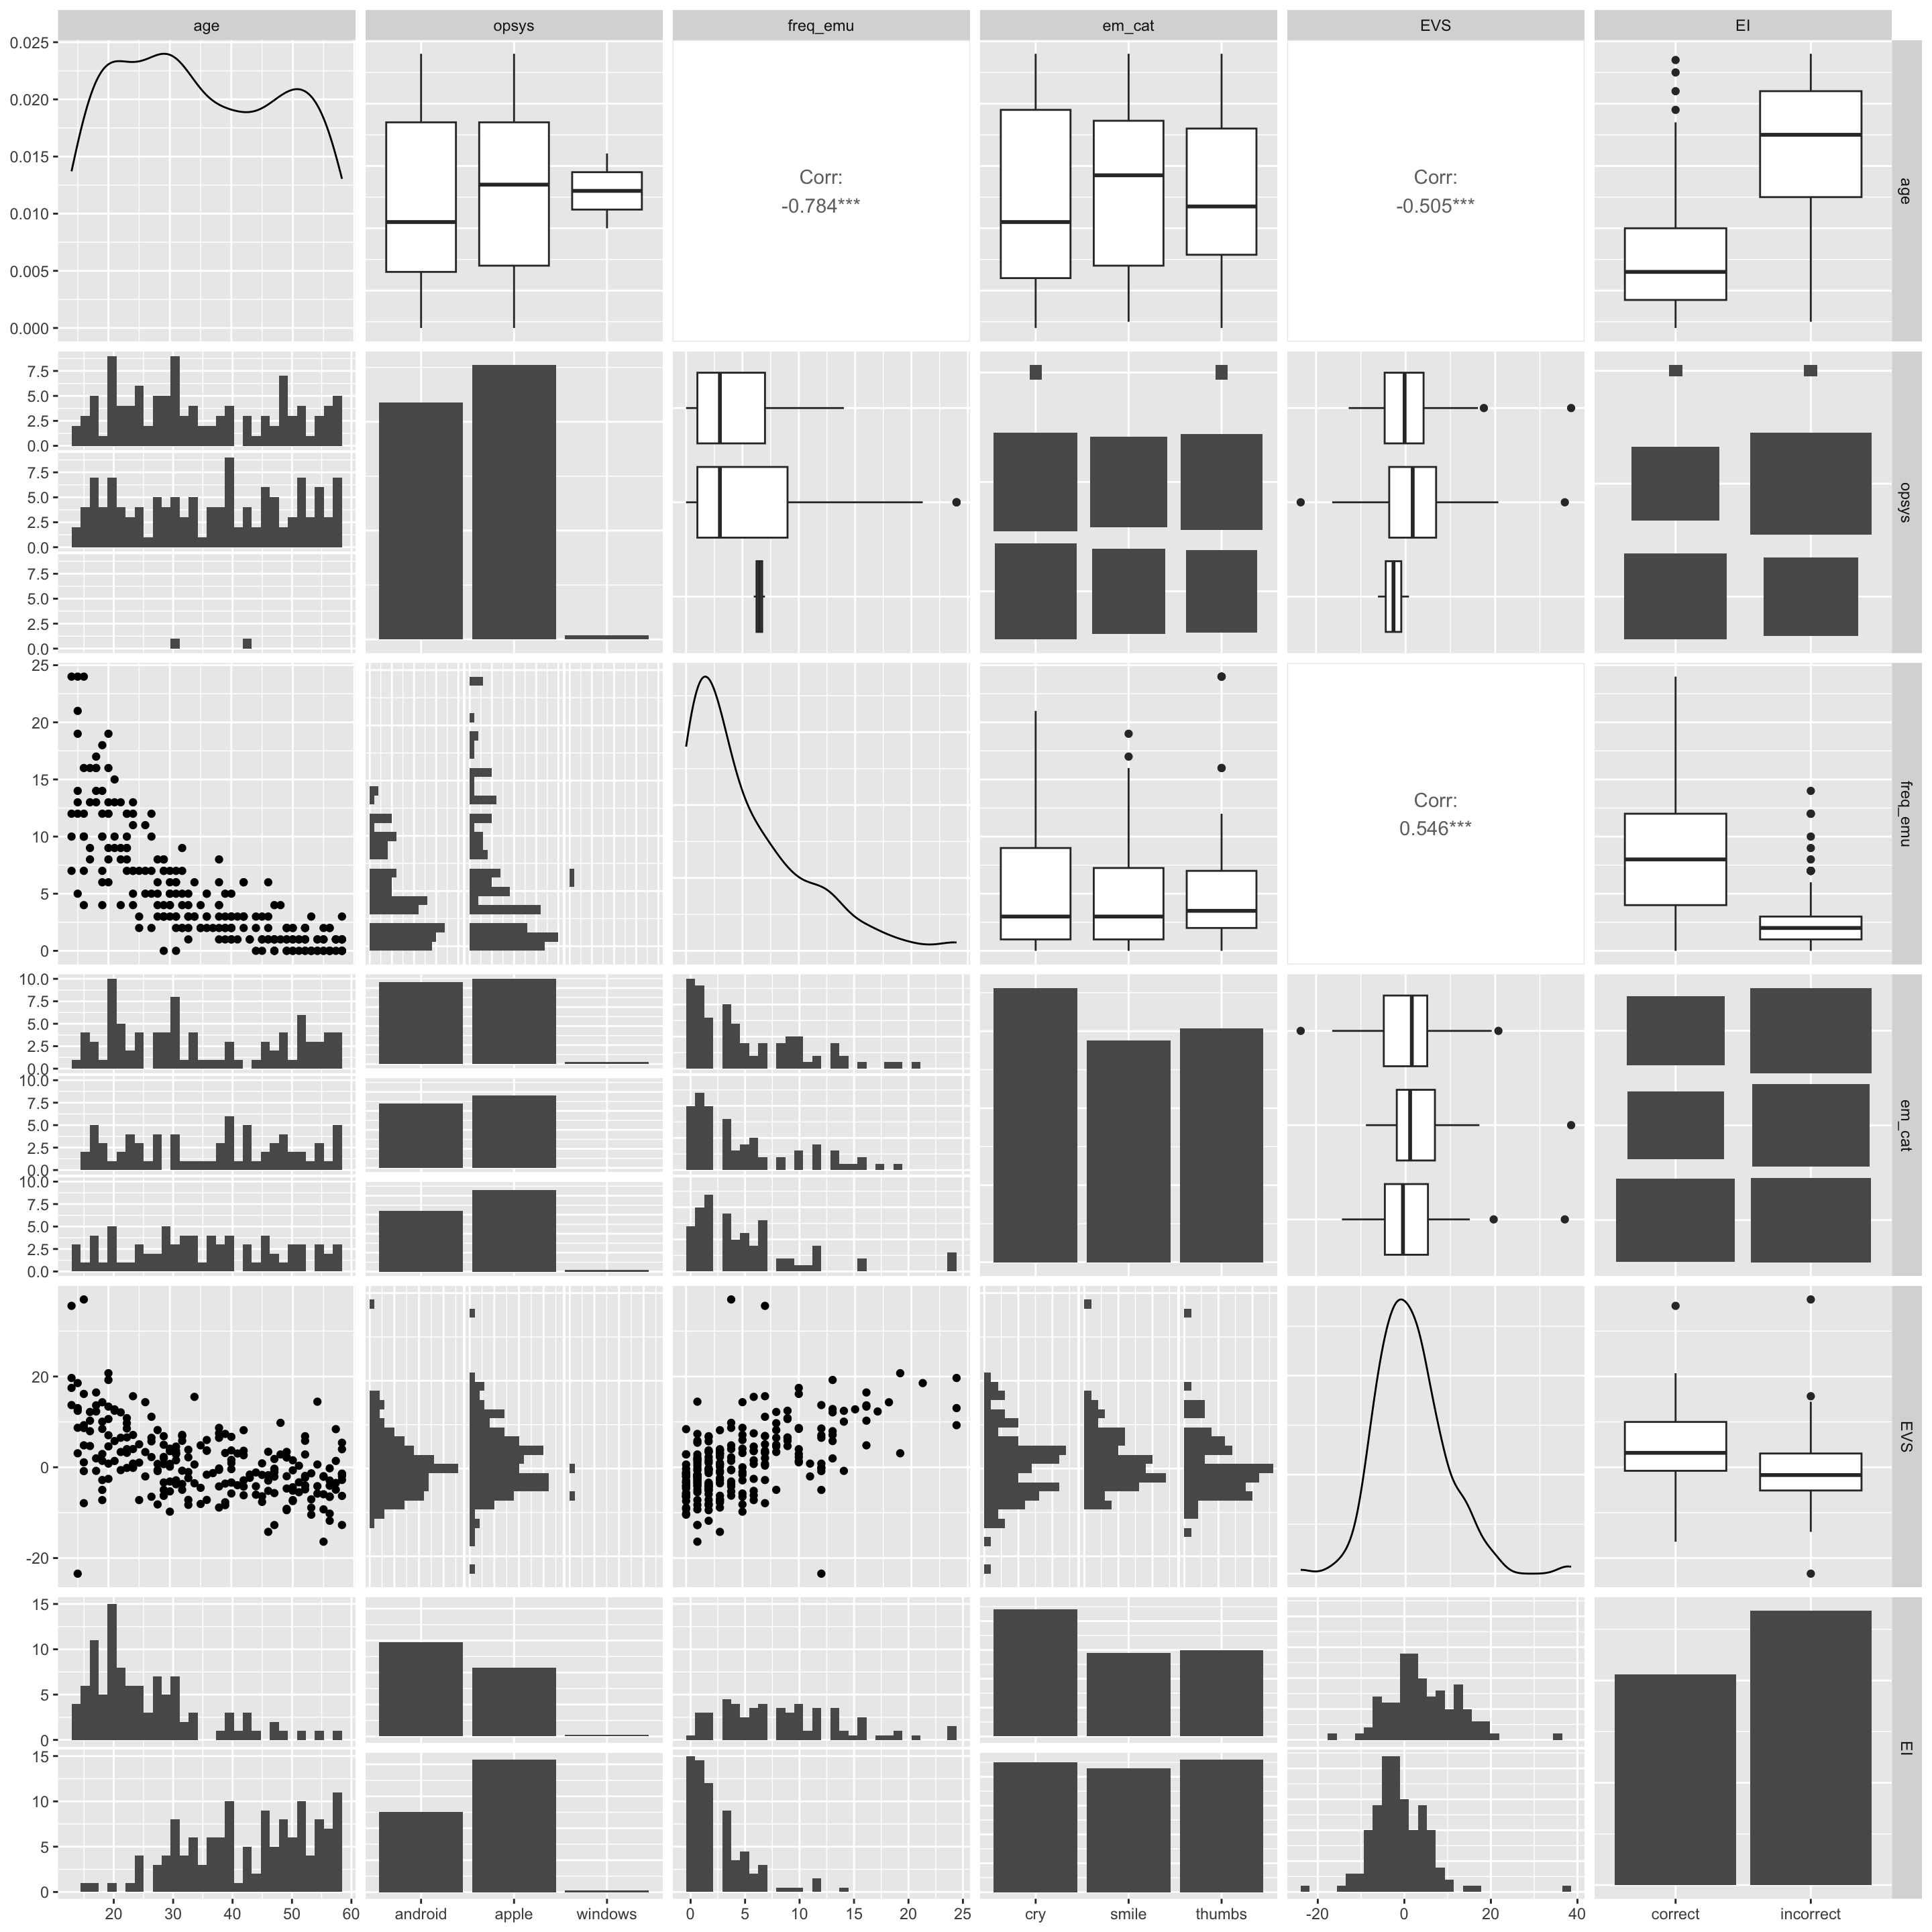
\includegraphics{Anteaters_Group_Project_files/figure-latex/unnamed-chunk-2-1.pdf}

\begin{figure}
\centering
\includegraphics{Anteaters_Group_Project_files/figure-latex/q3-desc-plots-1.pdf}
\caption{\label{fig:q3-desc-plots}Marginal Distributions and Relationships of Variables of Interest for Interpretation Accuracy}
\end{figure}

Given the binary outcome (correct vs.~incorrect interpretation; see Figure ), we fitted a multiple logistic regression model. We included the same predictors as the previous linear regression; frequency of emoji use first as its effect on interpreting emoji is already known, and additionally age as well as emoji category and the interaction between these to investigate if the effect of age on interpretation differs for the emoji being interpreted. Like the previous model, we mean-centered age, which estimates the coefficients and intercept at the mean age rather than age 0. Secondly, we used treatment coding (exact contrast coding in Table @ref cat-code-tab) for the emoji category since the three different kinds of emoji have no natural reference group. Each coefficient is then the difference between the mean level and the grand mean, and that all other coefficients are interpreted across levels rather than within a reference level. The final model has the following equation (note, E1 and E2 refers to the sum to zero coded variables in Table \ref{tab:cat-code-tab}):

\[
\log\left[ \frac {P(\operatorname{Emoji Interpretation} = \operatorname{correct})}{P(\operatorname{Emoji Interpretation} = \operatorname{incorrect})} \right] = \beta_0 + \beta_{1}(\operatorname{Emoji use frequency}) + \beta_{2}(\operatorname{Age_{mean-centered}}) + \beta_{3}·E_1 + \beta_{4}·E_2 + \beta_{5}(\operatorname{Age_{mean-centered}} \times \operatorname{E_1}) + \beta_{6}(\operatorname{Age_{mean-centered}} \times \operatorname{E_2})
\]

To answer the research question, we conduct the following tests. Firstly, an analysis of deviance is conducted using a \(\chi^2\) test to test if each predictor significantly reduces model deviance. Secondly, we investigate the associated regression coefficients of significant predictors. We examine their direction and significance using z-tests (\(\alpha\) = .05).

Before conducting these inferential tests, we examined the studentised (see Figure ) and standardised deviance residuals (see Figure @ref q3-stand-dev-res-plot)

\begin{table}

\caption{\label{tab:q3-dev-tab}Emoji Interpretation: Analysis of Deviance Table}
\centering
\begin{tabular}[t]{lllrrl}
\toprule
  & Df & Deviance & Residual Df & Residual Deviance & p-value\\
\midrule
Intercept-only &  &  & 236 & 324.49 & \\
Emoji use frequency & 1 & 96.51 & 235 & 227.97 & < 0.001\\
Age & 1 & 24.04 & 234 & 203.94 & < 0.001\\
Emoji category & 2 & 1.91 & 232 & 202.03 & 0.385\\
Age:Emoji category & 2 & 7.12 & 230 & 194.91 & 0.028\\
\bottomrule
\end{tabular}
\end{table}

As shown in Table x,

\label{tab:q3-tab-model} Logistic Regression Model

~

Correct Emoji Interpretation

Predictors

Odds Ratio

std. Error

95 \% CI

z-statistic

p-value

Intercept

0.32

0.11

0.16~--~0.63

-3.22

0.001

Emoji use frequency

1.12

0.08

0.99~--~1.29

1.68

0.092

Age

0.87

0.03

0.82~--~0.92

-4.47

\textless0.001

Emoji {[}😭{]}

1.64

0.42

0.99~--~2.76

1.91

0.056

Emoji {[}🙂{]}

1.09

0.30

0.63~--~1.90

0.31

0.760

Age:Emoji {[}😭{]}

1.06

0.03

1.00~--~1.12

2.02

0.044

Age:Emoji {[}🙂{]}

1.04

0.03

0.98~--~1.10

1.19

0.235

Observations

237

Deviance

194.912

log-Likelihood

-97.456

Across emoji categories, the chance of correctly interpreting an emoji was. Which emoji was interpreted and emoji use frequency predicted no significant change in this likelihood. Age, on the other hand, reduced the predicted probability of correct interpretation; for each year above the sample mean, \textbf{xx}.

\begin{figure}
\centering
\includegraphics{Anteaters_Group_Project_files/figure-latex/q3-model-plots-1.pdf}
\caption{\label{fig:q3-model-plots}Predicted Probability of Correct Emoji Interpretation for (A) Emoji Use Frequency and (B) Age for Each Emoji Tested}
\end{figure}

see \ref{fig:q3-model-plots}

\hypertarget{appendix-supplementary-tables-and-figures}{%
\section{Appendix: Supplementary Tables and Figures}\label{appendix-supplementary-tables-and-figures}}

\hypertarget{data-preparation-1}{%
\subsection{Data Preparation}\label{data-preparation-1}}

\begin{table}
\centering
\begin{tabular}{l|r|l|r|l|r|l|l}
\hline
Name & Age & Operating system & Emoji use frequency & Emoji category & Emotional valence score & Emoji Interpretation & Reason for exlcusion\\
\hline
Beatrix Potter & 28 & Apple & 6 & upside-down face & -4.0211784 & incorrect & Emoji not in study materials is reported\\
\hline
Thomas Burnet & 1 & Android & 6 & slightly smiling face & 13.1687730 & incorrect & Impossible or unlikely age\\
\hline
Joseph Priestley & NA & Apple & 10 & slightly smiling face & -1.1653997 & correct & Age is missing\\
\hline
Robert Bunsen & -99 & Apple & 6 & thumbs up & 0.4258727 & incorrect & Impossible or unlikely age\\
\hline
Luigi Galvani & 43 & Apple & -4 & slightly smiling face & 3.7097433 & incorrect & Impossible frequency value (negative) is reported\\
\hline
\end{tabular}
\end{table}

\begin{figure}
\centering
\includegraphics{Anteaters_Group_Project_files/figure-latex/ini-pairs-panels-1.pdf}
\caption{\label{fig:ini-pairs-panels}Marginal Distributions and Between-Variable Relationships for Pre-Processed Data}
\end{figure}

\hypertarget{data-description-1}{%
\subsection{Data Description}\label{data-description-1}}

\hypertarget{the-emotional-effect-of-emojis}{%
\subsection{The Emotional Effect of Emojis}\label{the-emotional-effect-of-emojis}}

\begin{table}

\caption{\label{tab:cat-code-tab}Emoji Category Treatment Contrast Coding Scheme}
\centering
\begin{tabu} to \linewidth {>{\raggedright}X>{\raggedleft}X>{\raggedleft}X}
\toprule
  & E1 & E2\\
\midrule
Loudly crying face & 1 & 0\\
Slightly smiling face & 0 & 1\\
Thumbs up & -1 & -1\\
\bottomrule
\end{tabu}
\end{table}

\hypertarget{accuracy-of-emoji-interpretation}{%
\subsection{Accuracy of Emoji Interpretation}\label{accuracy-of-emoji-interpretation}}

\begin{figure}
\centering
\includegraphics{Anteaters_Group_Project_files/figure-latex/q3-stand-dev-res-plot-1.pdf}
\caption{\label{fig:q3-stand-dev-res-plot}Standardised Deviance Residuals for Logistic Regression Model}
\end{figure}

\#Exam Numbers: ``B155926, B239086, B239979, B244840, B246814''

\hypertarget{notes-for-report-to-be-deleted}{%
\section{Notes for report (to be deleted)}\label{notes-for-report-to-be-deleted}}

(JMEP; 16/11/2023 - midnight zoomies) found this cool way of generating lm equation :0 equatiomatic

(JMEP; 16/11/2023 - midnight zoomies) Would be helpful if we could do all our code for each section in one chunk. Then we can call tables/figures where we need them and refer to numbers in inline code. Inline code example: NA (there is an NA in age, booo)

(JMEP; 16/11/2023 - midnight zoomies) I looked into age. There is one NA, one person who is -100 years old and one that is 1 year old. I think we can reliably remove them (done in emoji\_clean). There are also a bunch (23 to be exact) that are under 18 (between 14 and 17), whom I am not sure if we should remove??
I also noticed some other unusual stuff. Frequency ratings below 0, and a typo in ``Apple'' for one of the operating systems (``Appple''). There are also only two Windows users which isn't really helpful in terms of analysis - might wanna exclude them.

\#Code to possibly be deleted:
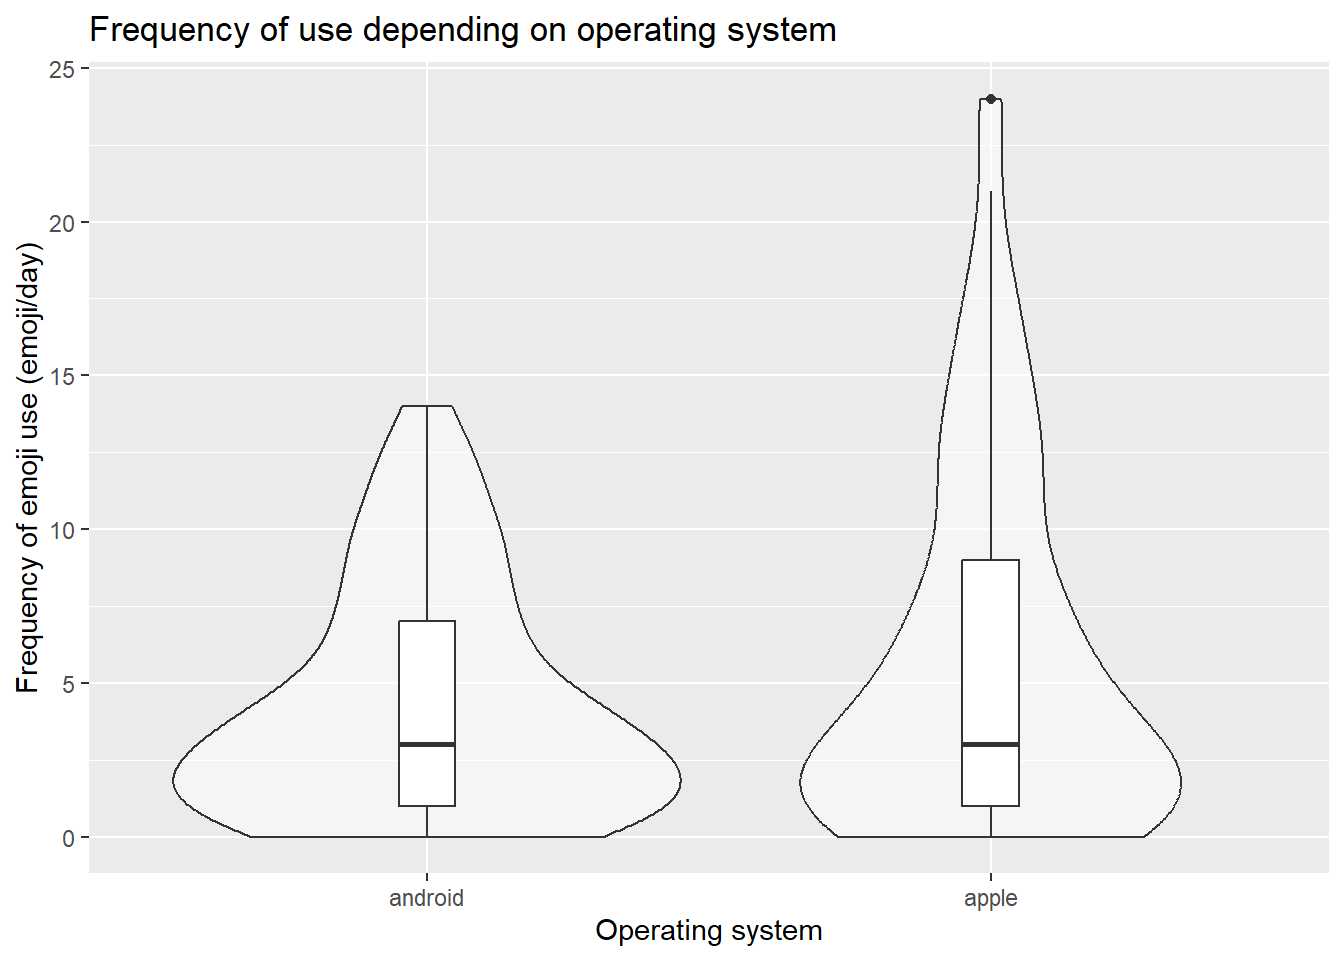
\includegraphics{Anteaters_Group_Project_files/figure-latex/unnamed-chunk-4-1.pdf}

\#probably to delete but just in case
For each emoji category, we found no significant difference between the observed proportions of Apple and Android users, and a hypothesised set of equal proportions. The results for each emoji category are as follows: loudly crying face emoji {[}😭{]}: \emph{n} = 88, \emph{proportion\textsubscript{Apple}} = 51.14 \%, \emph{proportion\textsubscript{Android}} = 48.86 \%; \(\chi^2\) (1) = 0.05, \emph{p} = 0.831; slightly smiling face emoji {[}🙂{]}: \emph{n} = 72, \emph{proportion\textsubscript{Apple}} = 52.78 \%, \emph{proportion\textsubscript{Android}} = 47.22 \%; \(\chi^2\) (1) = 0.22, \emph{p} = 0.637; thumbs up emoji {[}👍{]}: \emph{n} = 75, \emph{proportion\textsubscript{Apple}} = 57.33 \%, \emph{proportion\textsubscript{Android}} = 42.67 \%; \(\chi^2\) (1) = 1.61, \emph{p} = 0.204.

\end{document}
